\documentclass{article}
\usepackage[T1]{fontenc}
\usepackage[utf8]{inputenc}
\usepackage[margin=2cm]{geometry}
\usepackage{graphicx}
\usepackage{parskip}

\title{Zadanie 3 - Raport}
\author{Jan Stusio}
\date{Kwiecień 2024}

\begin{document}

\maketitle

\section{Wstęp}

Celem zadania jest zaimplementowanie algorytmu MinMax i alpha pruning dla gry w kółko i krzyżyk.


\section{Implementacja}

Przygotowałem konsolową grę w kółko i krzyżyk. 
Gracz wykonuje tylko decyzje Maxa, a komputer ruchy Mina. 
Przed każdym ruchem (poza początkowym) w konsoli wyświetla się najlepszy ruch dla gracza.

\textbf{Przebieg gry:}\\

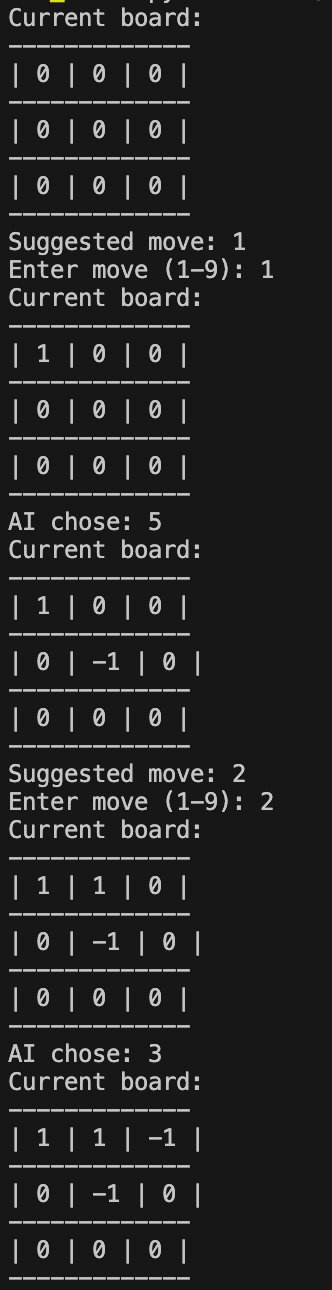
\includegraphics[width=4cm, height=10cm]{Screenshot 2024-04-15 at 21.58.35.png}
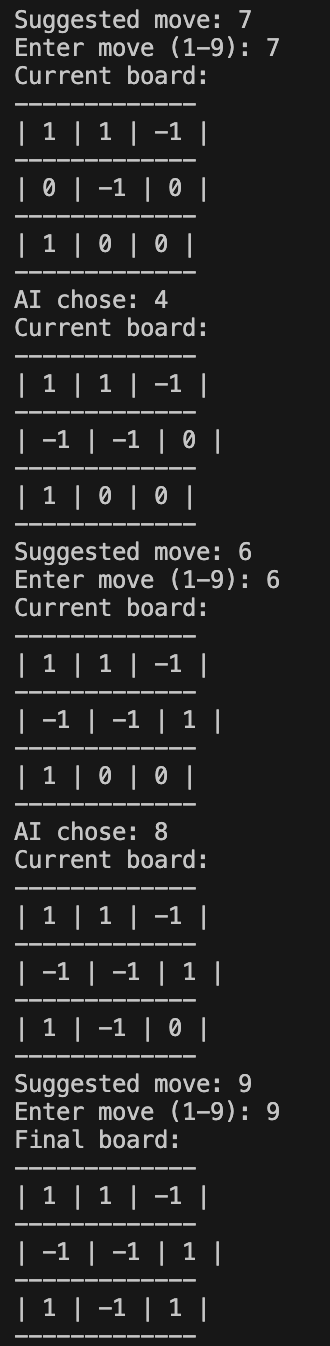
\includegraphics[width=4cm, height=10cm]{Screenshot 2024-04-15 at 21.58.19.png}


Algorytm MinMax zaimplementowałem w klasie o tej samej nazwie zgodnie z sygnaturami sugerowanymi w treści zadania
(za wyjątkiem akcji) zgodnie z rekurencyjnym pseudokodem podanym na wykładach. Nie implementowałem heurystyki.

Gra zaimplementowana jest w klasie TikTakToe oraz pliku main.py

\pagebreak

\section{Badania}

Badałem:

\quad 1. Liczbę odwiedzonych węzłów oraz głębokość drzewa dla wszystkich możliwych początkowych stanów gry (9 opcji) oraz 3 wybranych stanów „ze środka” gry

\quad 2. Jak alpha pruning wpływa na głębokość drzewa i liczbę odwiedzanych węzłów

\quad 3. Zależności czasu wykonania algorytmu dla pojedynczego ruchu w zależności od postępu w grze z i bez alpha pruningu

\section{Wyniki badań}

\subsection{Odwiedzanie węzłów i głębokość drzewa}

Badane stany "środka" gry:\\

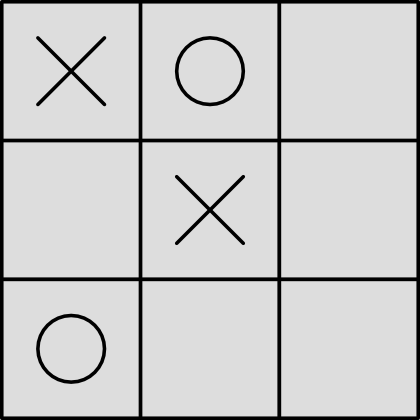
\includegraphics[width=5cm, height=5cm]{midgamestate1.png}
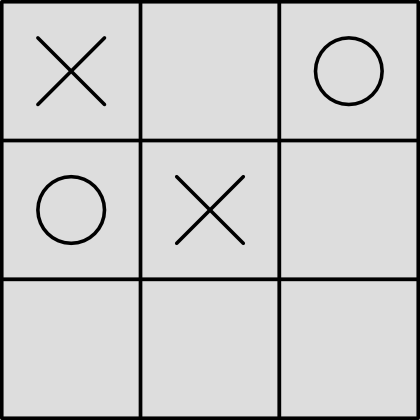
\includegraphics[width=5cm, height=5cm]{midgamestate2.png}
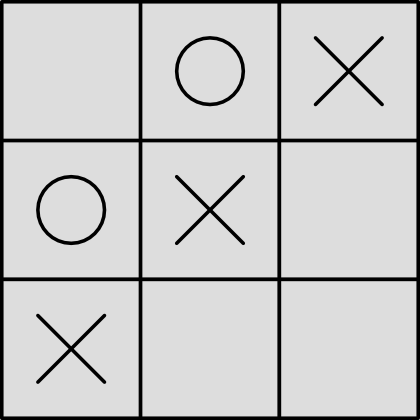
\includegraphics[width=5cm, height=5cm]{midgamestate3.png}
\\
MinMax - Nodes Visited: 48437, Execution Time: 1.75285s\\
Alpha-Beta - Nodes Visited: 1812, Execution Time: 0.06629s\\
MinMax - Nodes Visited: 55577, Execution Time: 2.33112s\\
Alpha-Beta - Nodes Visited: 1487, Execution Time: 0.10822s\\
MinMax - Nodes Visited: 48437, Execution Time: 1.79786s\\
Alpha-Beta - Nodes Visited: 1909, Execution Time: 0.07017s\\
MinMax - Nodes Visited: 55577, Execution Time: 2.07119s\\
Alpha-Beta - Nodes Visited: 1581, Execution Time: 0.05934s\\
MinMax - Nodes Visited: 40721, Execution Time: 1.40812s\\
Alpha-Beta - Nodes Visited: 2184, Execution Time: 0.07787s\\
MinMax - Nodes Visited: 55577, Execution Time: 2.09316s\\
Alpha-Beta - Nodes Visited: 2159, Execution Time: 0.07972s\\
MinMax - Nodes Visited: 48437, Execution Time: 1.76408s\\
Alpha-Beta - Nodes Visited: 1961, Execution Time: 0.07022s\\
MinMax - Nodes Visited: 55577, Execution Time: 2.09480s\\
Alpha-Beta - Nodes Visited: 2499, Execution Time: 0.09042s\\
MinMax - Nodes Visited: 48437, Execution Time: 1.78922s\\
Alpha-Beta - Nodes Visited: 2165, Execution Time: 0.07634s\\
MinMax - Nodes Visited: 182, Execution Time: 0.00659s\\
Alpha-Beta - Nodes Visited: 97, Execution Time: 0.00359s\\
MinMax - Nodes Visited: 1, Execution Time: 0.00003s\\
Alpha-Beta - Nodes Visited: 1, Execution Time: 0.00003s\\
MinMax - Nodes Visited: 1, Execution Time: 0.00004s\\
Alpha-Beta - Nodes Visited: 1, Execution Time: 0.00004s\\
MinMax - Nodes Visited: 48437, Execution Time: 1.60270s\\
Alpha-Beta - Nodes Visited: 1812, Execution Time: 0.06079s\\
MinMax - Nodes Visited: 4016, Execution Time: 0.10060s\\
Alpha-Beta - Nodes Visited: 204, Execution Time: 0.00611s\\
MinMax - Nodes Visited: 1, Execution Time: 0.00001s\\
Alpha-Beta - Nodes Visited: 1, Execution Time: 0.00000s\\
MinMax - Nodes Visited: 1, Execution Time: 0.00000s\\
Alpha-Beta - Nodes Visited: 1, Execution Time: 0.00000s\\
MinMax - Nodes Visited: 1, Execution Time: 0.00000s\\
Alpha-Beta - Nodes Visited: 1, Execution Time: 0.00000s\\
MinMax - Nodes Visited: 1, Execution Time: 0.00000s\\
Alpha-Beta - Nodes Visited: 1, Execution Time: 0.00000s\\
MinMax - Nodes Visited: 1, Execution Time: 0.00001s\\
Alpha-Beta - Nodes Visited: 1, Execution Time: 0.00000s\\
MinMax - Nodes Visited: 1, Execution Time: 0.00000s\\
Alpha-Beta - Nodes Visited: 1, Execution Time: 0.00001s\\
MinMax - Nodes Visited: 1, Execution Time: 0.00000s\\
Alpha-Beta - Nodes Visited: 1, Execution Time: 0.00000s\\

\subsection{Pomiar czasu}

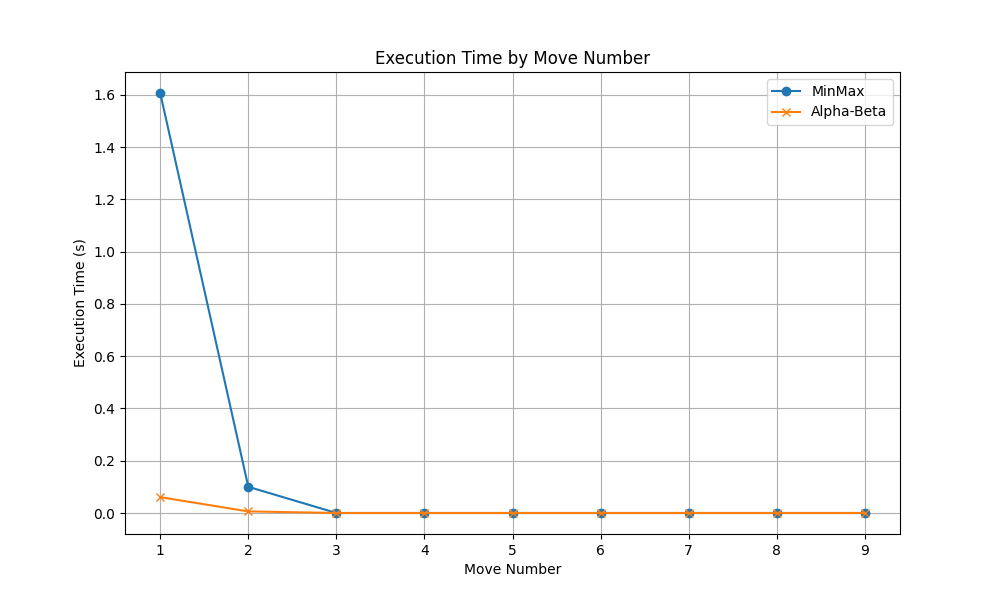
\includegraphics[width=7.7cm, height=6cm]{execution_time.png}


\section{Wnioski}

Czas wykonania algorytmu dla pojedynczego ruchu w zależności od postępu w grze bez alpha pruningu spada w miarę postępu gry, co jest zgodne z oczekiwaniami.
Dla alpha pruningu czas wykonania jest znacznie krótszy w początkowych stanach gry. W miarę postępu gry różnica w czasie wykonania dla obu algorytmów maleje, co jest zgodne z oczekiwaniami.
Głębokość drzewa dla alpha pruningu jest znacznie mniejsza niż dla MinMaxa bez niego, ale liczba odwiedzonych węzłów jest nieznacznie większa.

\end{document}
